\documentclass{article}

% Set basic page settings
\usepackage[hmargin=15mm, vmargin=15mm]{geometry}
\usepackage{fancyhdr}
% Allow for custom font sizes
\usepackage{anyfontsize}

% Set up a custom accent color
\usepackage{color}
\definecolor{slate}{rgb}{0.18,0.24,0.32}

% Used to include a headshot
\usepackage{graphicx}
\graphicspath{ {./images/} }

% Required for specification of custom fonts
\usepackage{fontspec}
\setmainfont[
  Path = ./fonts/,
  Extension = .otf,
  BoldFont = Erewhon-Bold,
  ItalicFont = Erewhon-Italic,
  BoldItalicFont = Erewhon-BoldItalic,
  SmallCapsFeatures = {Letters = SmallCaps}
]{Erewhon-Regular}

% Allow creation of hyperlinks formatted to the accent color
\usepackage{hyperref}
\hypersetup{urlcolor=slate, colorlinks=true}
\urlstyle{same}

% Set section titles to use accent color
\usepackage{sectsty}
\sectionfont{\color{slate}}

% Suppress section numbering
\setcounter{secnumdepth}{0}

% Use plain pages with no numbering or headers/footers
\pagestyle{empty}

% Stop paragraph indentation
\setlength\parindent{0pt}


% Amount to indent detail sections
\newlength{\detailindent}
\setlength{\detailindent}{15mm}

% Text width for detail sections
\newlength{\detailwidth}
\setlength{\detailwidth}{\textwidth}
\addtolength{\detailwidth}{-1.05\detailindent}

% Non-indenting itemized list for job achievements
\newenvironment{achievements}
  {\setlength{\leftmargini}{4mm}\begin{itemize}}
  {\end{itemize}}


\newcommand{\header}[9] {
  \parbox{0.75\textwidth} {
    {\fontsize{40}{48}\color{slate}\textbf{\href{https://github.com/lordjabez/resume}{#1}} \hspace{1mm} (he/him)}
    \begin{tabbing}
      \hspace{60mm}        \= \kill
      \\
      #2                   \> \url{#6} \\
      #3                   \> \url{#7} \\
      #4                   \> \url{#8} \\
      #5                   \> \url{#9} \\
    \end{tabbing}
  }
  \parbox{0.24\textwidth} {
    \begin{flushright}
      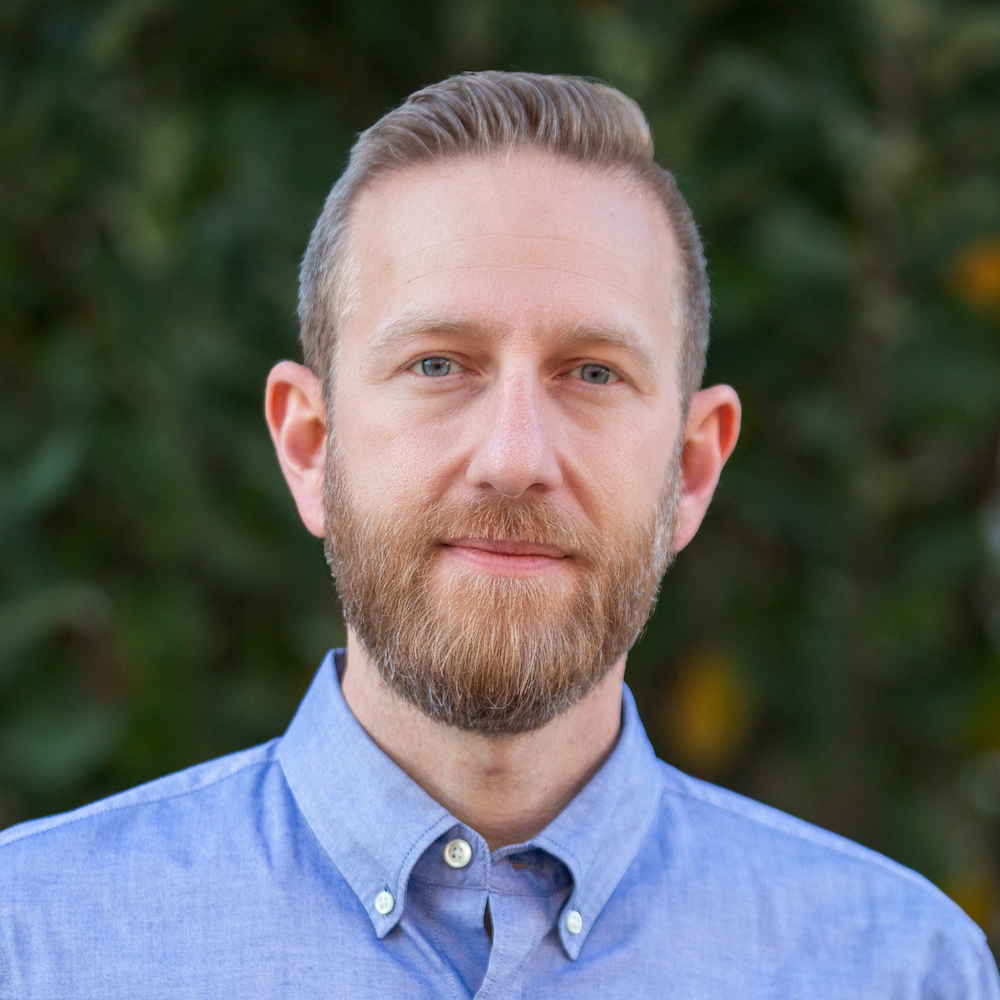
\includegraphics[height=40mm]{headshot}
    \end{flushright}
  }
  \vspace{-1mm}
}


\newcommand{\job}[5] {
  \begin{tabbing}
    \hspace{\detailindent} \= \kill
    \textbf{#2} \> #3 \\
    \hspace{3.33mm}\textbf{|}  \> \textit{#4} \\
    \textbf{#1} \> \\
  \end{tabbing}
  \vspace{-9mm}
  \hspace{\detailindent}
  \begin{minipage}{\detailwidth}
    #5
  \end{minipage}
  \vspace{2mm}
}


\newcommand{\skill}[2] {
  \begin{tabbing}
    \hspace{\detailindent} \= \kill
    \textbf{#1} \>   #2
  \end{tabbing}
}


\newcommand{\education}[3] {
  \begin{tabbing}
    \hspace{\detailindent} \= \kill
    \textbf{#1} \>   #2 \\
                \>\+ \textit{#3} \\
  \end{tabbing}
  \vspace{-7mm}
}


\newcommand{\credits} {
  \pagestyle{fancy}
  \renewcommand{\headrulewidth}{0pt}
  \renewcommand{\footrulewidth}{0pt}
  \cfoot {
    \footnotesize{\textit{Version \version. Built using LaTeX and Docker. Source code available at \url{https://github.com/lordjabez/resume}.}}
  }
}

\def\version{0.0.0}\input



\begin{document}


\header
  {Judson Neer}
  {16627 Deer Ridge Road}
  {San Diego, CA 92127-3446}
  {judson.neer@gmail.com}
  {937.902.7765}
  {https://linkedin.com/in/judsonneer}
  {https://github.com/lordjabez}
  {https://stackoverflow.com/u/2262968}
  {https://makingofthings.com}


\section{Profile}

Technologist building both systems and organizations that are secure, scaleable, cost-effective, and most of all, promote human flourishing. Well-versed in programming languages, cloud technologies, and people management. Experienced with the entire engineering lifecycle, from ideation and requirements design to architecture and implementation to sales and support. Also an avid runner, amateur musician, and owner of every iteration of the Raspberry Pi.


\section{Experience}

\job
  {2023}{Present}
  {Research Improving People's Lives}
  {Chief Technology Officer}
  {\begin{achievements}
    \item Lead the organization building secure, scalable, and cost-effective solutions for better government
    \item Responsible for the engineering team's budget, hiring, and culture, and delivery excellence
    \item Determine strategic technical investments that further the company's mission to improve people's lives
  \end{achievements}}

\job
  {2019}{2023}
  {Amazon Web Services}
  {Delivery Practice Manager}
  {\begin{achievements}
    \item Led the professional services team that built transformative solutions for US-based education and state \& local government customers
    \item Scaled the delivery organization from 8 to 40 people, mentoring both individual contributors and front-line managers, and participating in recruiting and ID\&E efforts within the group
    \item Collaborated with sales teams to book and then deliver several multi-million dollar projects in areas such as unemployment insurance, elections, health care, and online learning
    \item Published both internal and public-facing software packages and other technical artifacts (see Github link for details)
    \item Interviewed 180 candidates for both technical and non-technical roles across Amazon; was primary decision maker as a Bar Raiser in 60 of them, and mentored 6 others through the Bar Raiser training program
    \item Developed, documented, and drove adoption of a suite of internal automation tools used by dozens of teams Amazon-wide, saving the company millions of dollars annually
  \end{achievements}}

\pagebreak

\job
  {2018}{2019}
  {Votem Corp}
  {Chief Architect}
  {\begin{achievements}
    \item Led the team responsible for software architecture and design across a suite of election products, with a particular focus on security, modularity, scaleability, availability, and cost-effectiveness
    \item Spearheaded company-wide security initiatives such as LastPass and Yubikey adoption in order to build a culture of transparency, integrity, and customer success
    \item Served the election industry by participating in the NIST Cybersecurity and Interoperability groups, and by chairing the DHS Election Infrastructure Sector Coordinating Council's Cybersecurity Working Group
  \end{achievements}}

\job
  {2014}{2018}
  {Everyone Counts, Inc}
  {Director Of Engineering}
  {\begin{achievements}
    \item Guided the engineering team through a stressful and prolonged acquisition, with no voluntary resignations during the process
    \item Provided technical and organizational leadership for a 25 person development team, regularly applying Conway's Law so the resultant products had the desired architecture
    \item Hired and then led a 6 person team that architected, implemented, deployed, and maintained an online voting system that used modern cryptographic techniques, and was scaleable to 10M+ voters with multi-zone deployments; system enjoyed over 99.998\% uptime during its 18 months of operation, and was used for the largest online election in the United States as of September 2017
    \item Maintained a legacy online voting system used by several high-profile clients
    \item Migrated a legacy voter registration web application to open-source operating systems and databases, saving \$100,000 annually in software licenses
  \end{achievements}}

\job
  {2001}{2014}
  {Northrop Grumman Corp}
  {Senior Software Engineer}
  {\begin{achievements}
    \item Championed a continuous integration process that reduced the build/test/deploy cycle from multiple hours to less than one minute
    \item Designed and implemented generic HTTP REST APIs and a common Android user interface for multiple heterogeneous radio systems, which increased operator effeciency and reduced setup errors
    \item Built a web-based communication planning tool for ground and airborne radios, which allowed warfighters to maximize comm-link effectiveness while minimizing risk
    \item Invented a technique for generating real-time flight path updates optimized for changing mission constraints (e.g. aircraft performance, flight time, threat envelopes, weather), which won the Northrop Grumman Strategic Intellectual Property Award
    \item Developed a moving map display for displaying terrain, navigation aids, threats, and other tactical information
  \end{achievements}}

\job
  {2000}{2001}
  {Grange Insurance}
  {Software Engineer}
  {\begin{achievements}
    \item Built an internal web application that allowed rapid access to the customer database
    \item Integrated a ZIP code lookup API that saved the data entry team several minutes per claim
  \end{achievements}}

\pagebreak


\section{Entrepreneurship}

\job
  {2019}{2019}
  {KNOWiNK, LLC}
  {Indepedent Consultant}
  {\begin{achievements}
    \item Architected the cloud deployment of a voter registration platform, optimizing for security, availability, performance, and cost
    \item Implemented a complete CI/CD pipeline using infrastructure-as-code and scaleable compute
    \item Collaborated with outside security teams (e.g. DHS) to ensure monitoring and compliance requirements were met
    \item Trained the in-house engineering team on cloud technologies and best practices
  \end{achievements}}

\job
  {2016}{2019}
  {Boxmaeker, LLC}
  {Co-Founder}
  {\begin{achievements}
    \item Built a device that communicates to a variety of weighing scale brands, publishing their measurements over Internet of Things protocols
    \item Used cloud infrastructure to record data, collect status information, and push software updates to on-site devices, greatly simplifying maintenance
    \item Developed a cross-platform mobile app for display and control of device data
    \item Implemented a mobile B2B app for a third-party supplier, generating \$500K of sales to date
    \item At exit sold company's intellectual property to hardware manufacturer for integration into their marquee product line
  \end{achievements}}


\section{Certifications}

\education
  {2020}
  {Amazon Web Services}
  {Certified Data Analytics - Specialty}

\education
  {2020}
  {Amazon Web Services}
  {Certified Security - Specialty}

\education
  {2019}
  {Amazon Web Services}
  {Certified Solutions Architect - Professional}

\education
  {2019}
  {Amazon Web Services}
  {Certified DevOps Engineer - Professional}


\section{Education}

\education
  {2013}
  {San Diego State University, San Diego, California, 3.92 GPA}
  {Advanced Certificate, Web And Mobile Applications Development}

\education
  {2001}
  {Cedarville University, Cedarville, Ohio, 3.96 GPA}
  {Bachelor of Science, Computer Science and Mathematics}


\section{}

\credits


\end{document}
